\section{Teilaufgabe 25}
\begin{aufgabe}
    Versuchen Sie jetzt den Regler so zu programmieren, dass Sie den I-Anteil 
    des Reglers isolieren könnten. Führen Sie die gleichen Simulationen durch 
    wie vorher und beobachten Sie den I-Anteil.
\end{aufgabe}
\begin{figure}[h!]
    \centering
    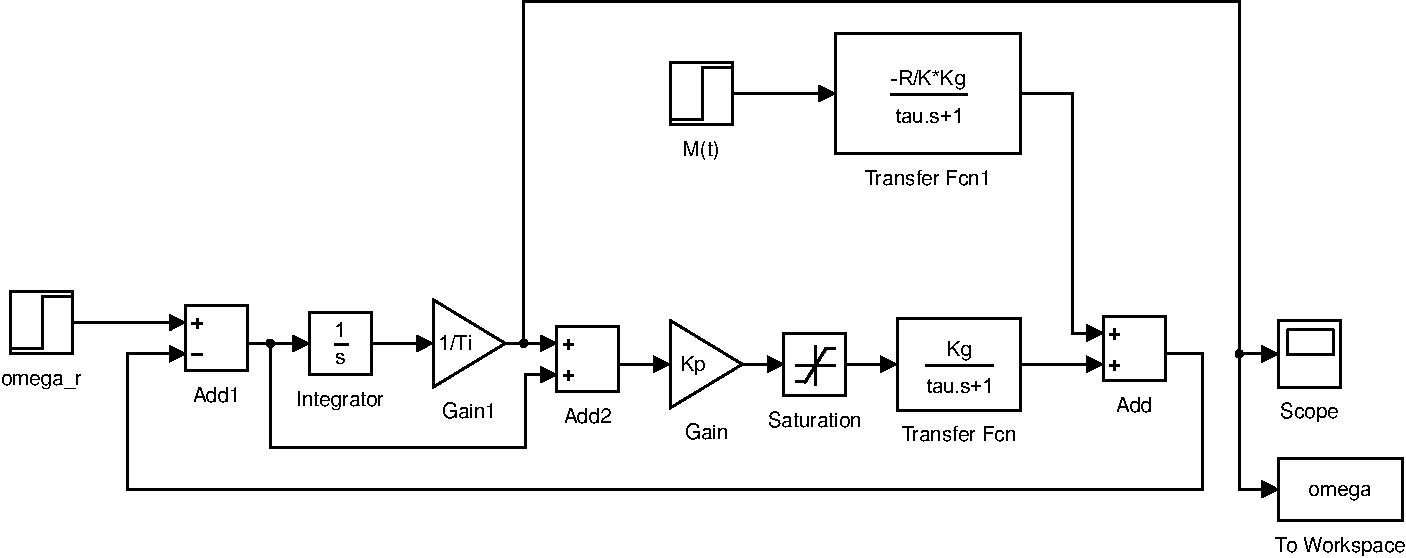
\includegraphics[width=0.6\textwidth]{25/regler_sat_isep.pdf}
    \caption{Regler in Simulink}
    \label{fig:25}
\end{figure}
\begin{figure}[h!]
    \centering
    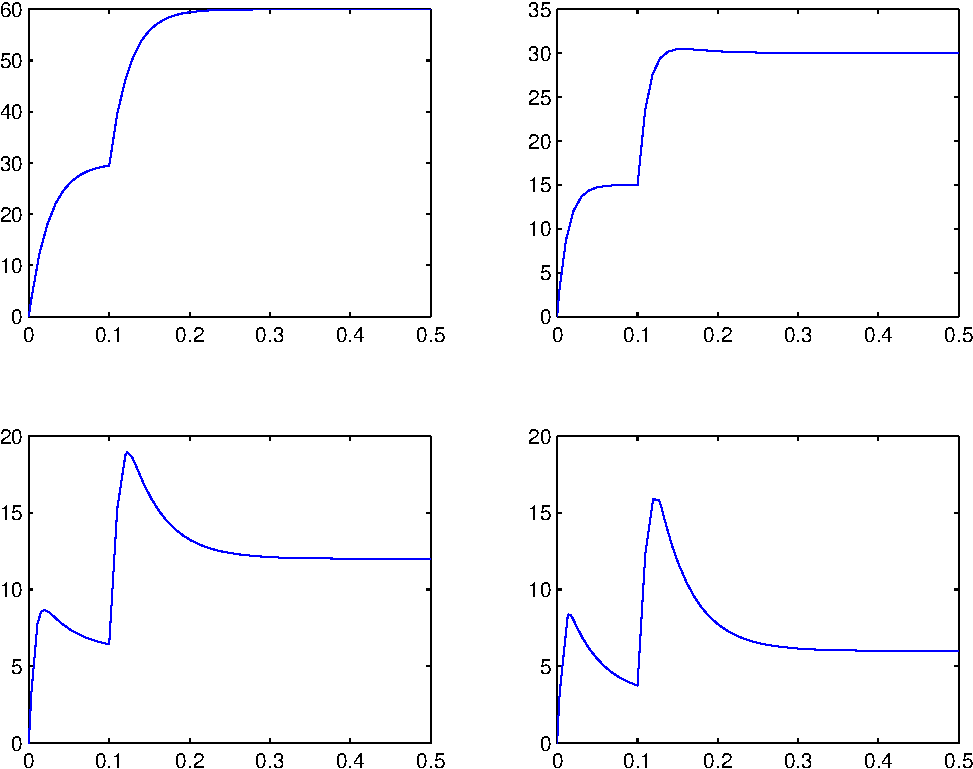
\includegraphics[width=0.6\textwidth]{25/regler_sat_isep_plot.pdf}
    \caption{Simulationsergebnis}
    \label{fig:25plot}
\end{figure}
\lstinputlisting{25/regler_sat_isep.m}
